\documentclass{beamer}
\beamertemplatenavigationsymbolsempty

\usepackage[utf8]{inputenc}
\usepackage[ngerman]{babel}
\usepackage{graphicx}
\usepackage{pdfpages}
\usepackage{hyperref}
\usepackage{qrcode}
\usepackage{eurosym}

\title{Fachschaftsvorstellung}
\subtitle{(extra informative edition)}

\begin{document}
	%\maketitle
	\begin{frame}
		\centering
		
\includegraphics[width=0.8\textwidth]{pictures/fsilogo_neu.pdf}
		\maketitle
	\end{frame}
	
	\begin{frame}{Wer sind wir?}
		\begin{figure}
			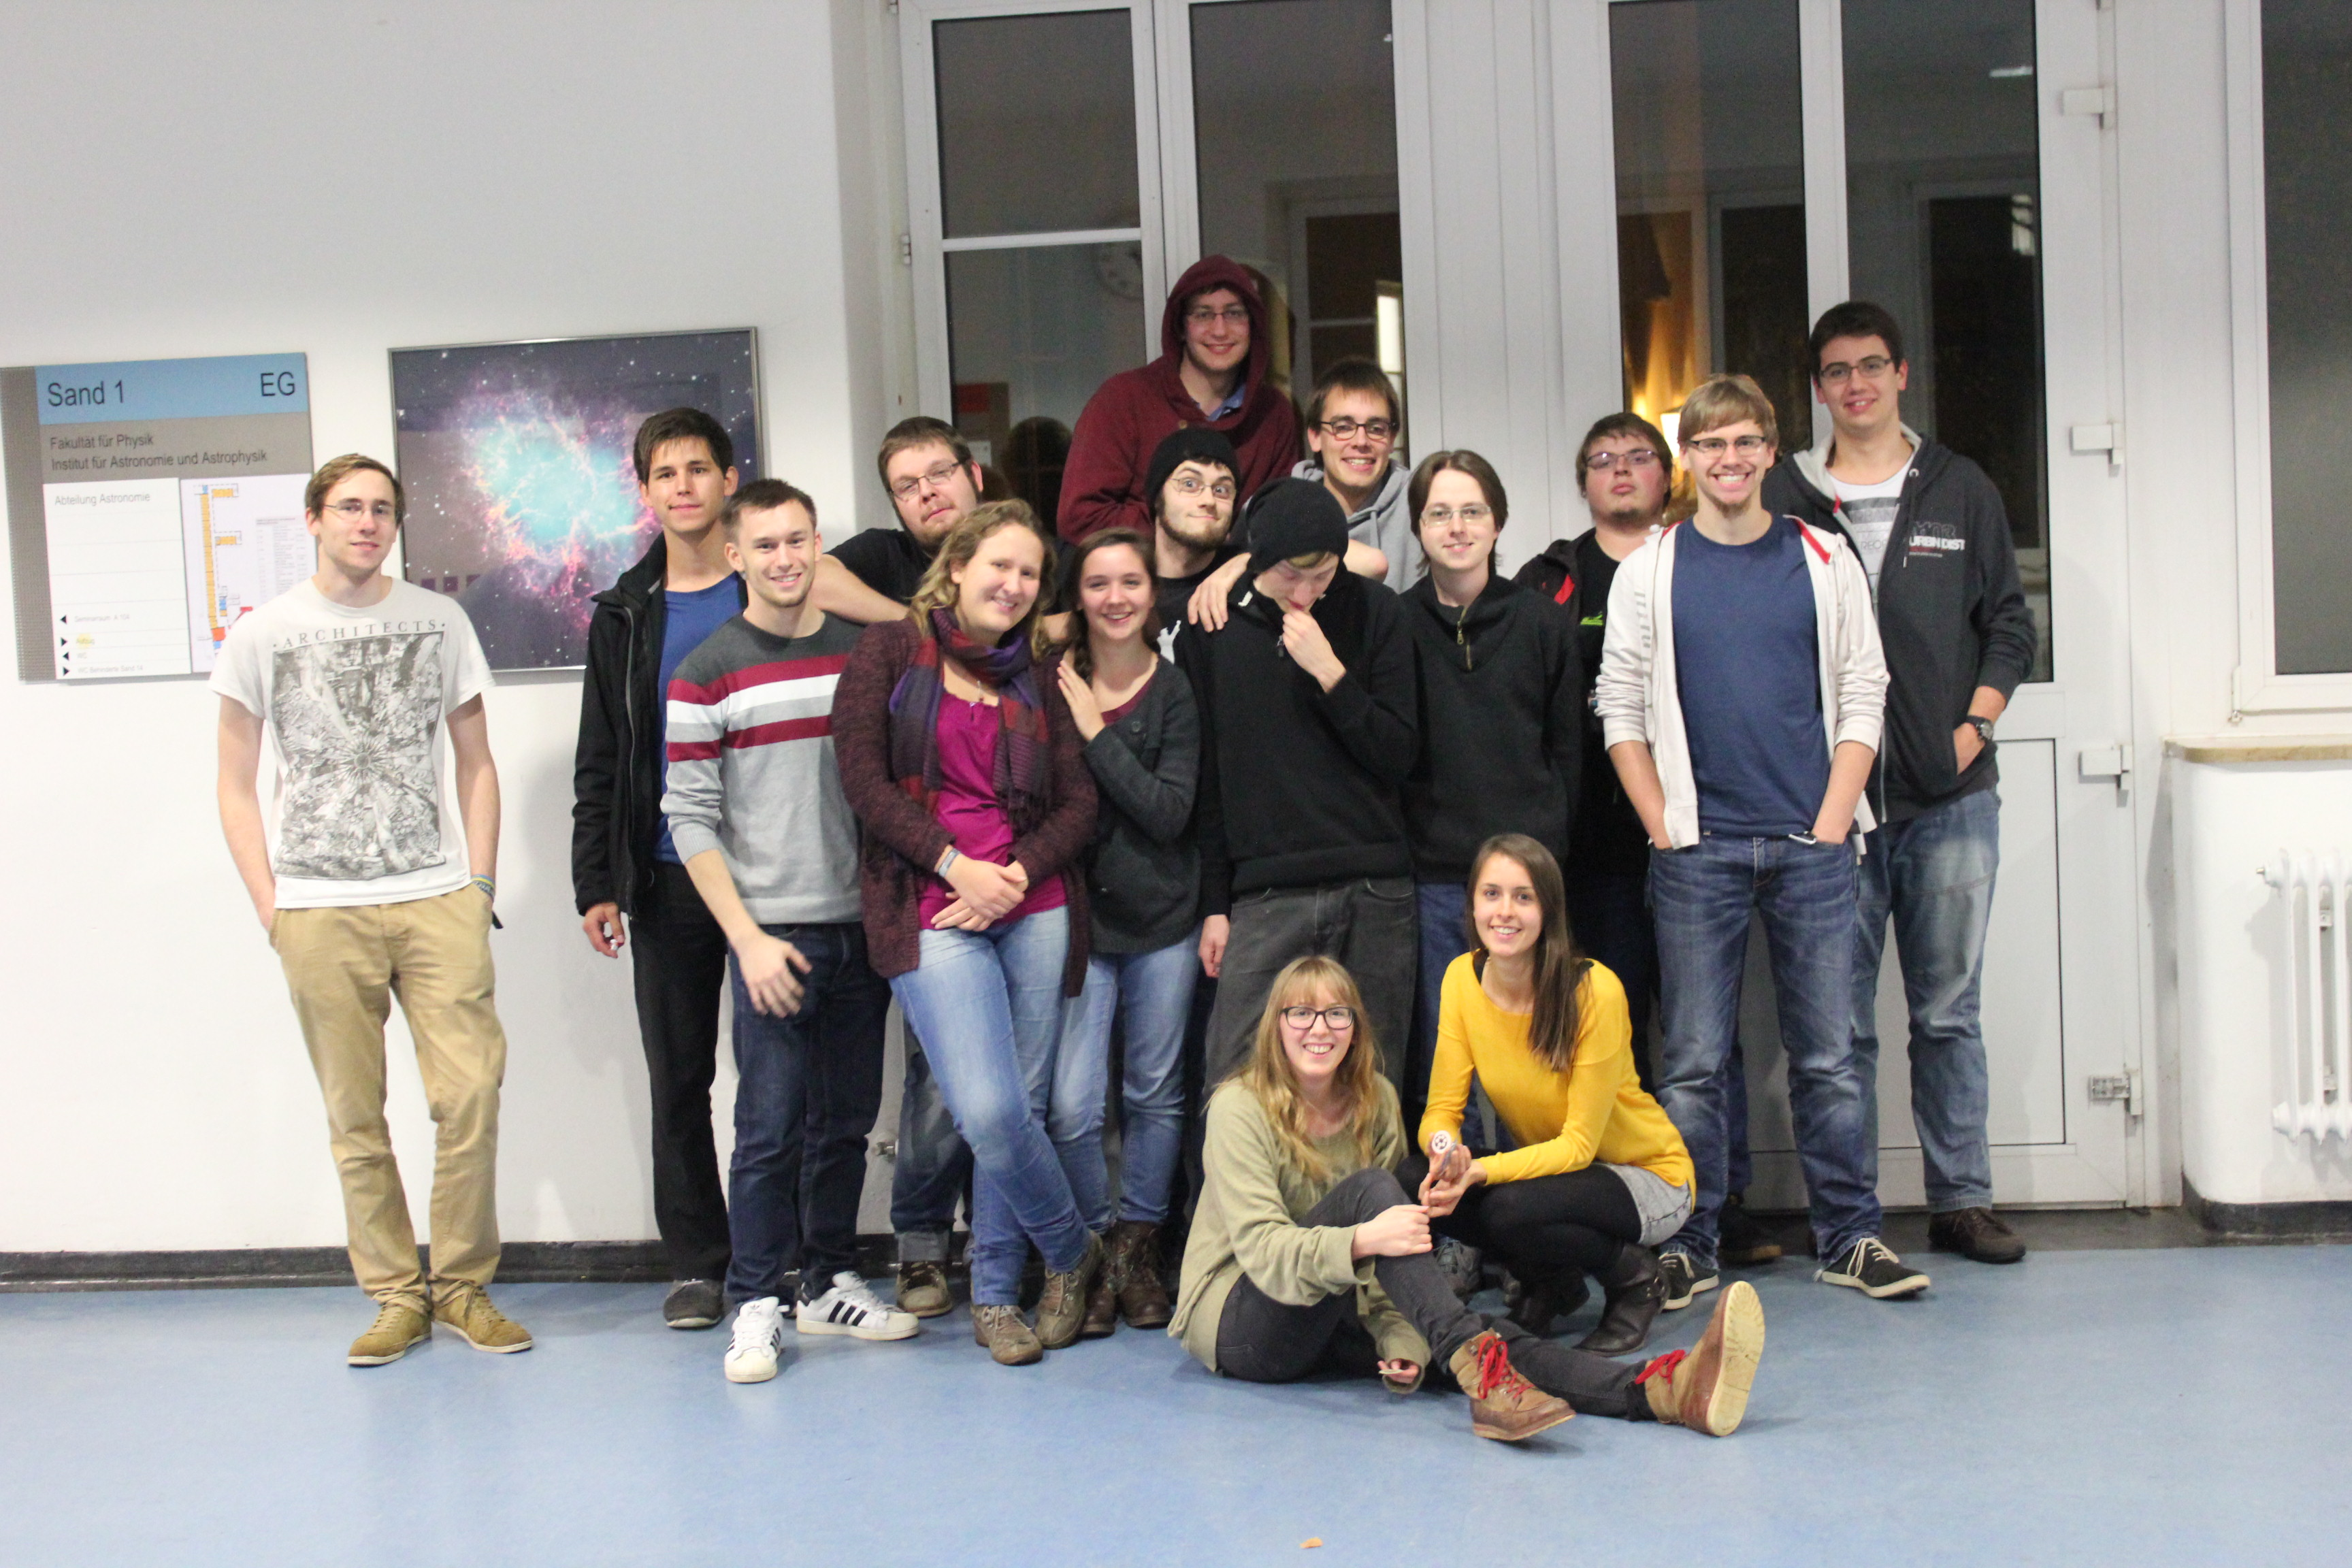
\includegraphics[width=0.9\textwidth]{pictures/fachschaft.jpg}
		\end{figure}
	\end{frame}
	
	\begin{frame}{Was machen wir?}
		\begin{figure}
			%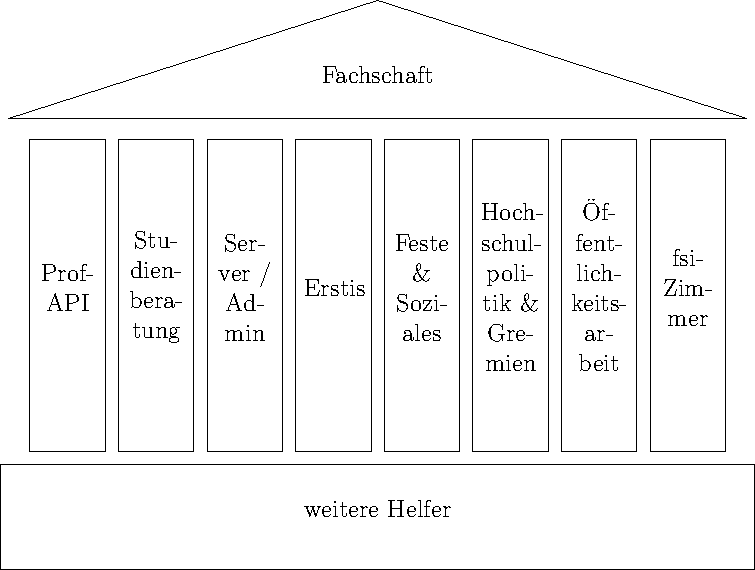
\includegraphics[width=0.9\textwidth]{pictures/selbstverstaendnis.pdf}
		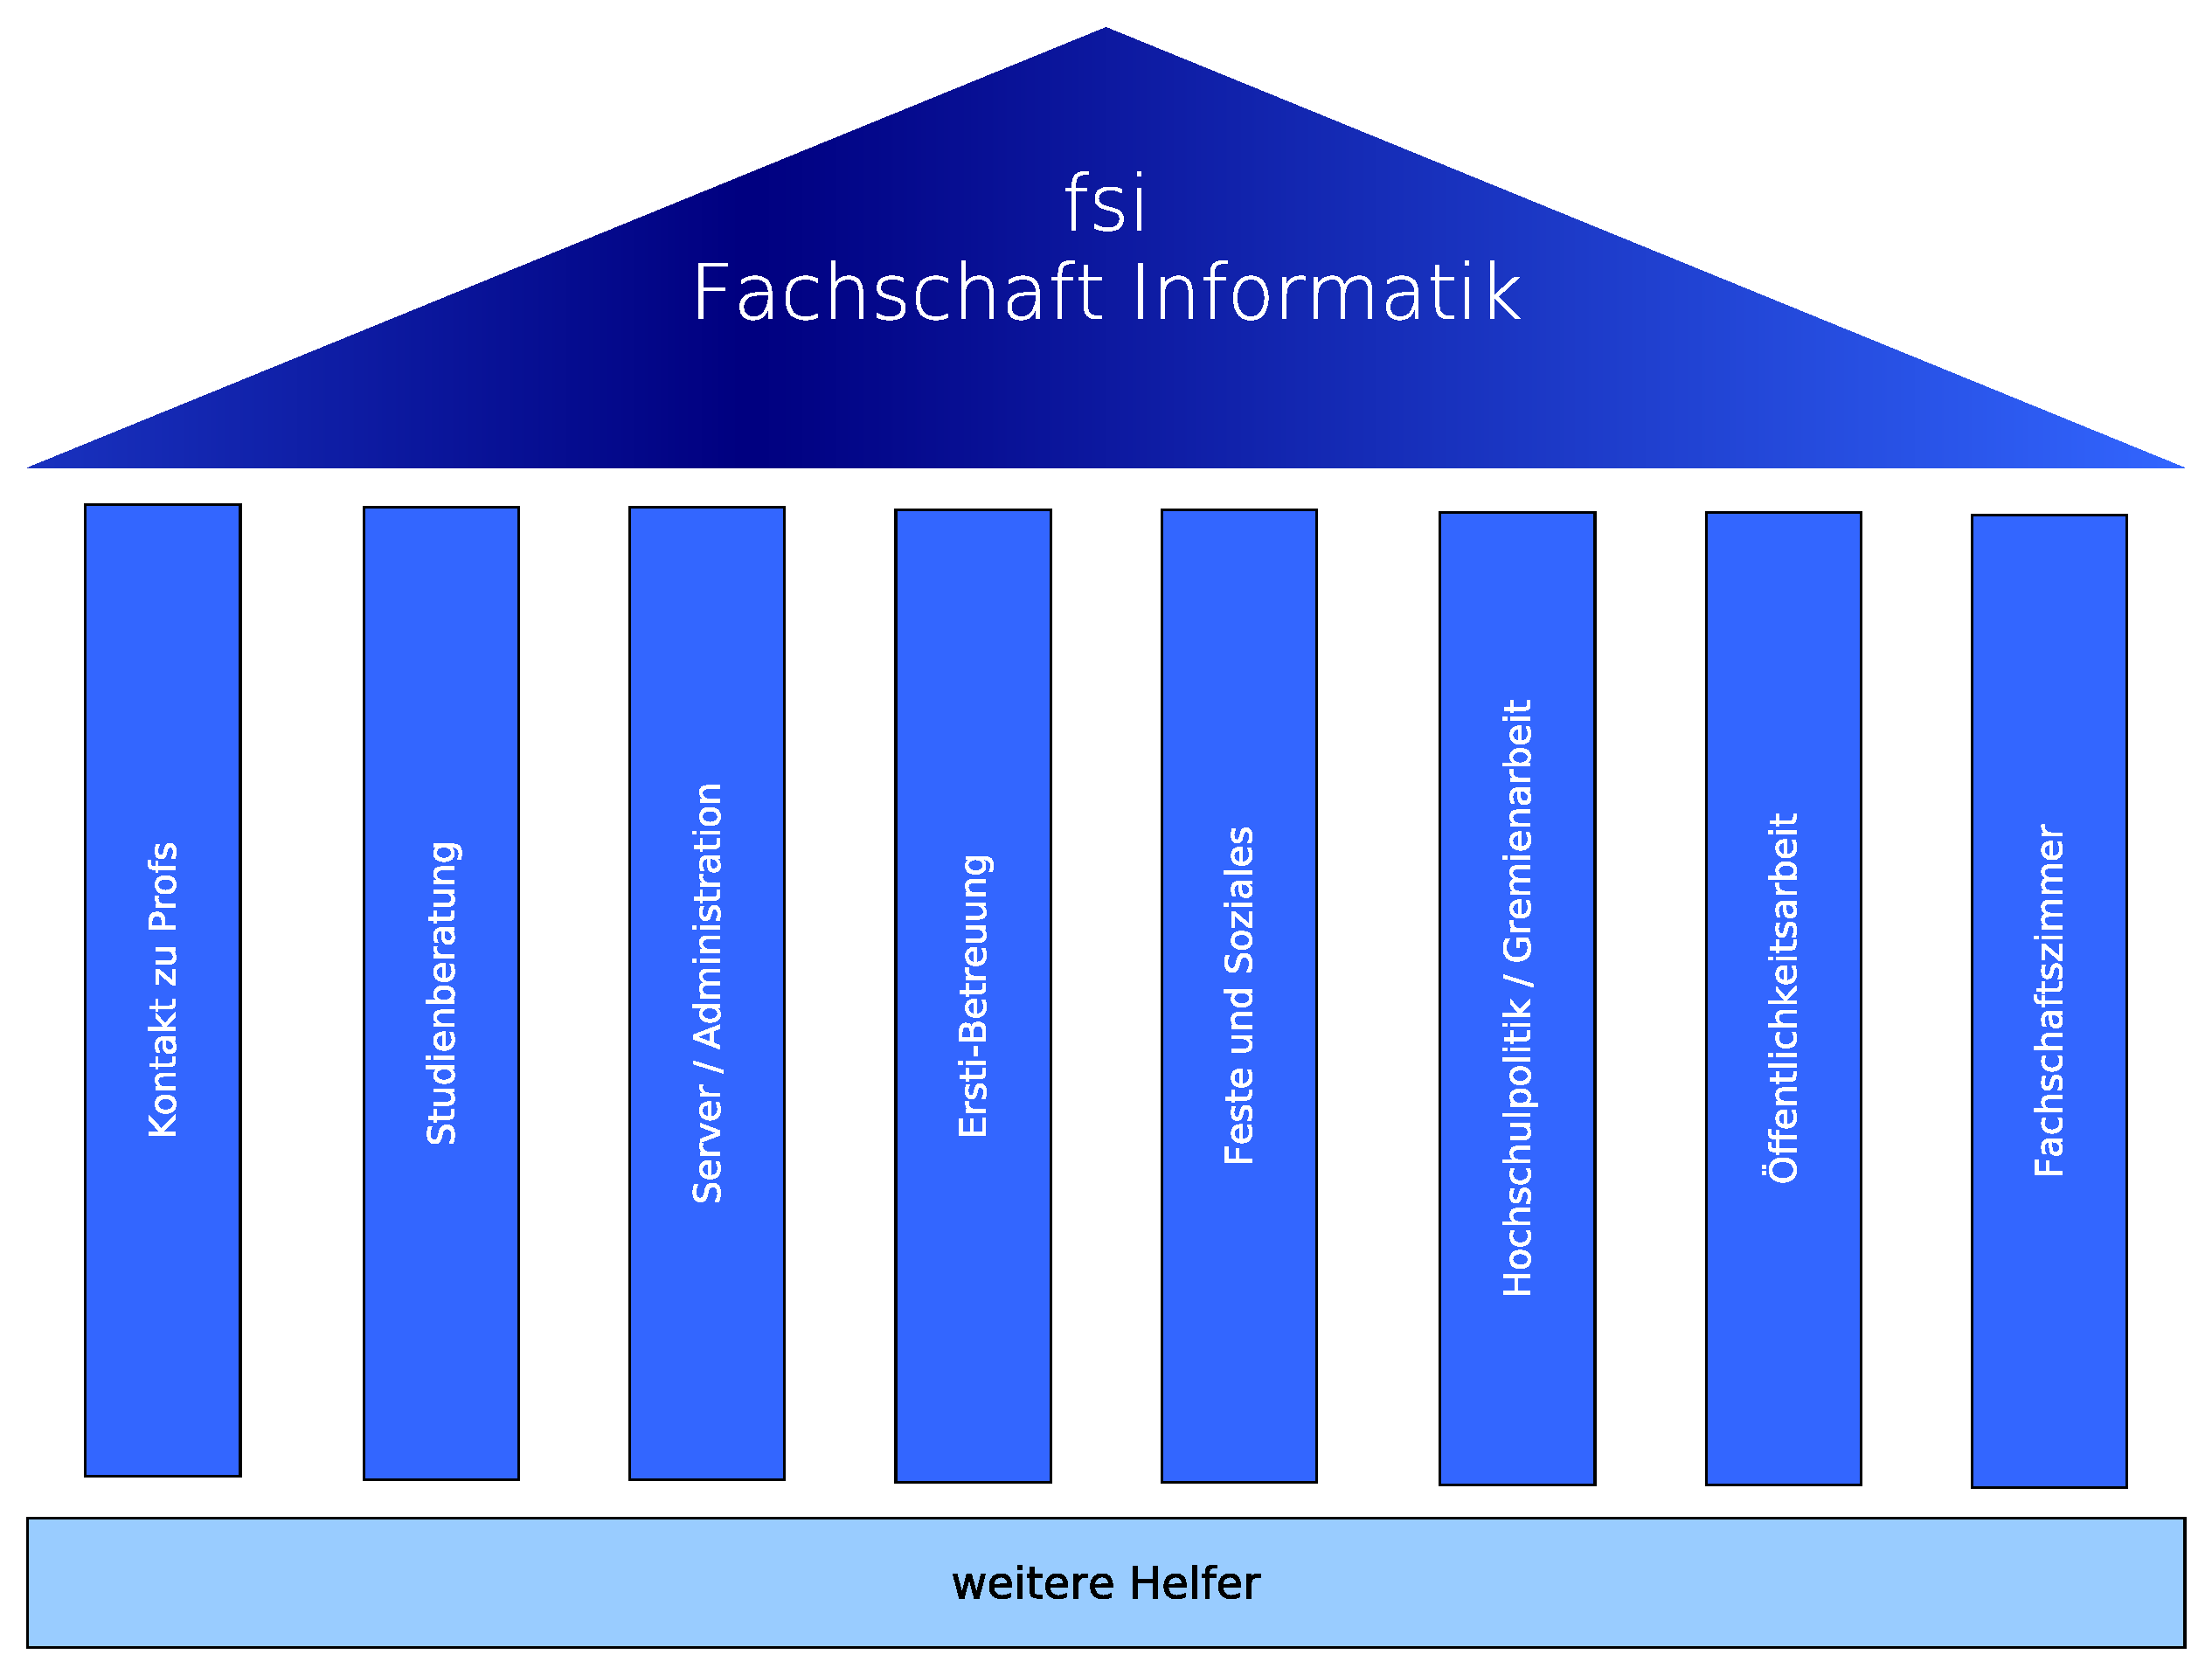
\includegraphics[width=0.9\textwidth]{pictures/fsi_saeulen.pdf}
		\end{figure}
	\end{frame}
 	
	\begin{frame}{Kontakt zu Profs}
		\begin{itemize}
			\item stehen in engem Kontakt mit der Professorenschaft
			\item können Probleme daher gut ansprechen
			\item (und meistens auch beheben)
			\item monatliche Treffen mit dem Fachbereich, um Problemen vorzubeugen
			\item[$\Rightarrow$] Wir brauchen euren Input!\\Also kommt zu uns, wenn ihr Probleme habt!
		\end{itemize}
	\end{frame}
	
	\begin{frame}{Studienberatung}
		\begin{itemize}			
			\item \textbf{Informatik \& Bioinformatik}\\			
			Beraterin: Jessica Wolz \& Vanessa Kirchner\\
			E-Mail: studienberatung[@]informatik[.]uni-tuebingen[.]de
			
			\item \textbf{Kognitionswissenschaft}\\	
			Berater: Paul Fischer \& Christian Secker\\
			E-Mail: kogni-beratung[@]fsi[.]uni-tuebingen[.]de
			
			\item \textbf{Medieninformatik}\\
			Berater: Vanessa Kirchner\\
			E-Mail: medieninformatik[@]uni-tuebingen[.]de\\
			
			\item \textbf{Medizininformatik}\\			
			Beraterin: Marie Gauder\\
			E-Mail: medizininformatik[@]uni-tuebingen[.]de
			
		\end{itemize}
	\end{frame}

	\begin{frame}{Server \& Administration}
		\begin{itemize}			
			\item Betreiben und Warten von verschiedener Infrastruktur
			\begin{itemize}
				\item Mailinglisten
				\item Website
				\item Prüfungsprotokolleinterface (PPI)
				\item Verkaufssystem
			\end{itemize}
			\item Usermanagement
			\item Entwicklung und Betrieb von Tools zur Fachschaftsarbeit
		\end{itemize}
	\end{frame}
	
	\begin{frame}{Server \& Administration}
	\framesubtitle{Mailinglisten}
		\begin{columns}
			\begin{column}{.5\textwidth}
				\textbf{*-InformatikerInnen:}
				\small
				\begin{itemize}
					\item info-studium 
					\item info-talk
					\item info-jobs
					\item sport
				\end{itemize}
			\end{column}
			\begin{column}{.5\textwidth}
				\textbf{Kognis:}\\
				\small
				\begin{itemize}
					\item kogwiss 
					\item versuche
					\item info-studium
					\item psycho-studium
				\end{itemize}

			\end{column}
		\end{columns}
		\vfill
		\textbf{Anmeldung:} Mail ohne Betreff und Inhalt an \$LISTNAME-subscribe@fsi.uni-tuebingen.de
	
	\end{frame}
	
	\begin{frame}{Erstsemesterveranstaltungen}
		\begin{itemize}
			\item Planung und Organisation der verschiedenen Veranstaltungen
			\begin{itemize}
				%\item Grillen, Frühstück, Kneipentour, etc.
				\item Grillen, Filmeabend, HowTo Studium, Kneipentour etc.
				%\item Erstiwochenende
			\end{itemize}
			\item Vorbereitung von Infos
			\begin{itemize}
				\item Brief
				\item Heft
			\end{itemize}
		\end{itemize}
	\end{frame}
			
	\begin{frame}{Partys \& Feste}
		\framesubtitle{ClubHausFest}
		\begin{columns}
			\begin{column}{.4\linewidth}
				\begin{itemize}
					\item jeden Donnerstag
					\item im Clubhaus 
					\item pro Fachschaft 1x im Semester
					\item CHF der Fachschaften Info/Kogni/Psycho am 04.05 (heute in einer Woche!)
				\end{itemize}
			\end{column}
			\begin{column}{.6\linewidth}
				
\includegraphics[width=\linewidth]{pictures/chf_jodel.jpg}
			\end{column}
		\end{columns}
	\end{frame}

	\begin{frame}{Partys \& Feste}
		\framesubtitle{Sommerfest}
		\begin{figure}
			%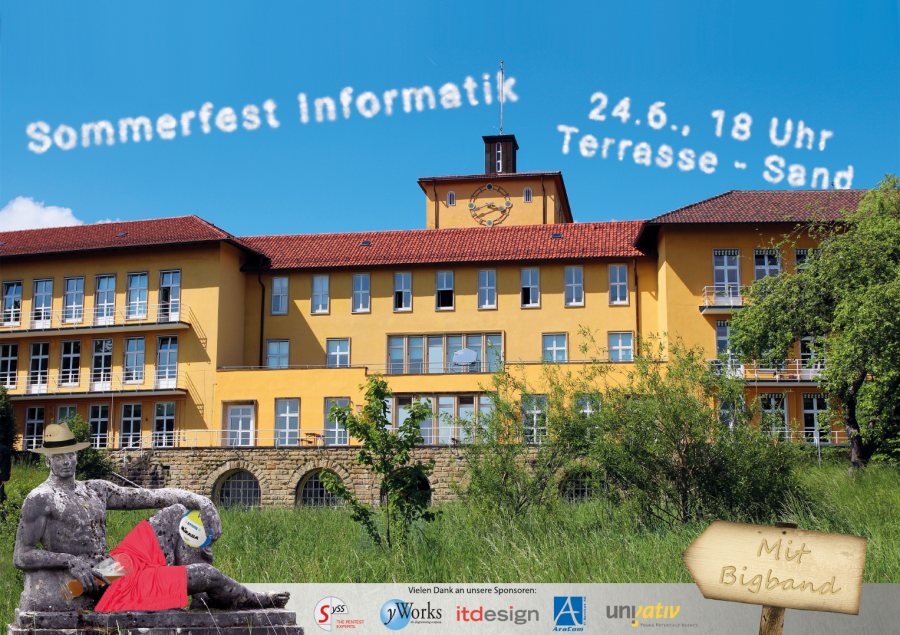
\includegraphics[width=0.9\textwidth]{pictures/sommerfest.png}
			
\includegraphics[width=0.9\textwidth]{pictures/sommerfest_platzhalter.png}
		\end{figure}
	\end{frame}
	
	\begin{frame}{Partys \& Feste}
		\framesubtitle{weiteres}
		\begin{itemize}
			\item Spieleabende
			\item LAN-Partys
			\item Pizza backen
		\end{itemize}
	\end{frame}
	
	\begin{frame}{Hochschulpolitik \& Gremien}
		\framesubtitle{Fakultätsrat}
	 	Entscheidet über
	 	\begin{itemize}
	 		\item Finanzen
	 		\item neue Professuren
	 		\item Forschung und Lehre
	 		\item Besetzung von Gremien
	 	\end{itemize}
	 	Wird jährlich von allen Studierenden der Fakultät gewählt (5 Studenten aus 11 Fachschaften).
	 \end{frame}
	
	\begin{frame}{Hochschulpolitik \& Gremien}
		\framesubtitle{Studienkommission}
	 	\begin{itemize}
	 		\item Wichtigstes Gremium für den Studienablauf
	 		\item Gestaltet Modulhandbuch
	 		\item Zwei Kommissionen:
	 			\begin{itemize}
	 				\item (Bio-, Medien-, Medizin-) Informatik
	 				\item Kognitionswissenschaft
	 			\end{itemize}
	 		\item 4 Profs, 2 Mitarbeiter, 4 Fachschaftler\\
	 	\end{itemize}
	 \end{frame}
	
	\begin{frame}{Hochschulpolitik \& Gremien}
		\framesubtitle{Prüfungsausschuss}
	 	\begin{itemize}
	 		\item Anerkennung von Studienleistungen
	 			\begin{itemize}
	 				\item Auslandssemester?
	 				\item ungewöhnliche Vorlesung für ein bestimmtes Modul?
	 				\item neues Nebenfach?
	 			\end{itemize}
	 		\item (theoretisch) PA für jeden Studiengang einzeln
	 		\item Fachschaftler mit beratender Stimme
	 	\end{itemize}
	 \end{frame}
	
	\begin{frame}{Hochschulpolitik \& Gremien}
		\framesubtitle{weitere studentische Gremien}
	 	\begin{itemize}
	 		\item StuRa - Studierendenrat (ersetzt AStA)
	 			\begin{itemize}
	 				\item Hochschulpolitisches Mandat
	 				\item kann Projekte unterstützen
	 				\item Gebühren zu Beginn des Semesters
	 			\end{itemize}
	 		\item Senat
	 		\item Vertreter fühlen sich meist einer Hochschulpolitischen Gruppe zugehörig:
	 			\begin{itemize}
	 				\item FSVV
	 				\item GHG
	 				\item JuSos
	 				\item RCDS
	 				\item ...
	 			\end{itemize}
	 	\end{itemize}
	 \end{frame}
	
	\begin{frame}{Fachschaftsarbeit}
		\framesubtitle{wie geht das?}
		\begin{columns}
			\begin{column}{.5\linewidth}
				\begin{itemize}
					\item einfach vorbeikommen und mitmachen ;-)
					\item regelmäßige Treffen im Fachschaftszimmer (Sand, Zimmer C125)
					\item nächstes Treffen: \\Donnerstag 27.04. 18:30 Uhr
					\item teilweise weitere Treffen zu Teilbereichen der Fachschaftsarbeit
					\item Kogni-Treffen: \emph{folgt}
					\item Kommt vorbei!
				\end{itemize}
			\end{column}
			\begin{column}{0.5\linewidth}
				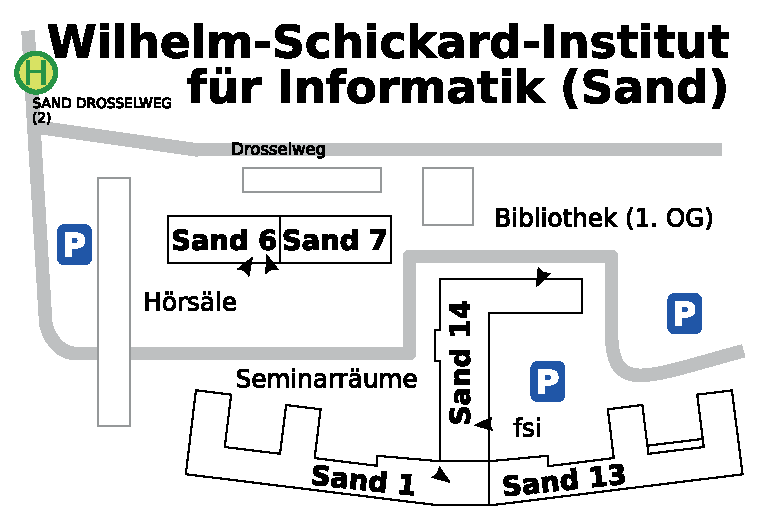
\includegraphics[width=\linewidth]{pictures/uebersicht_sand.pdf}\\
				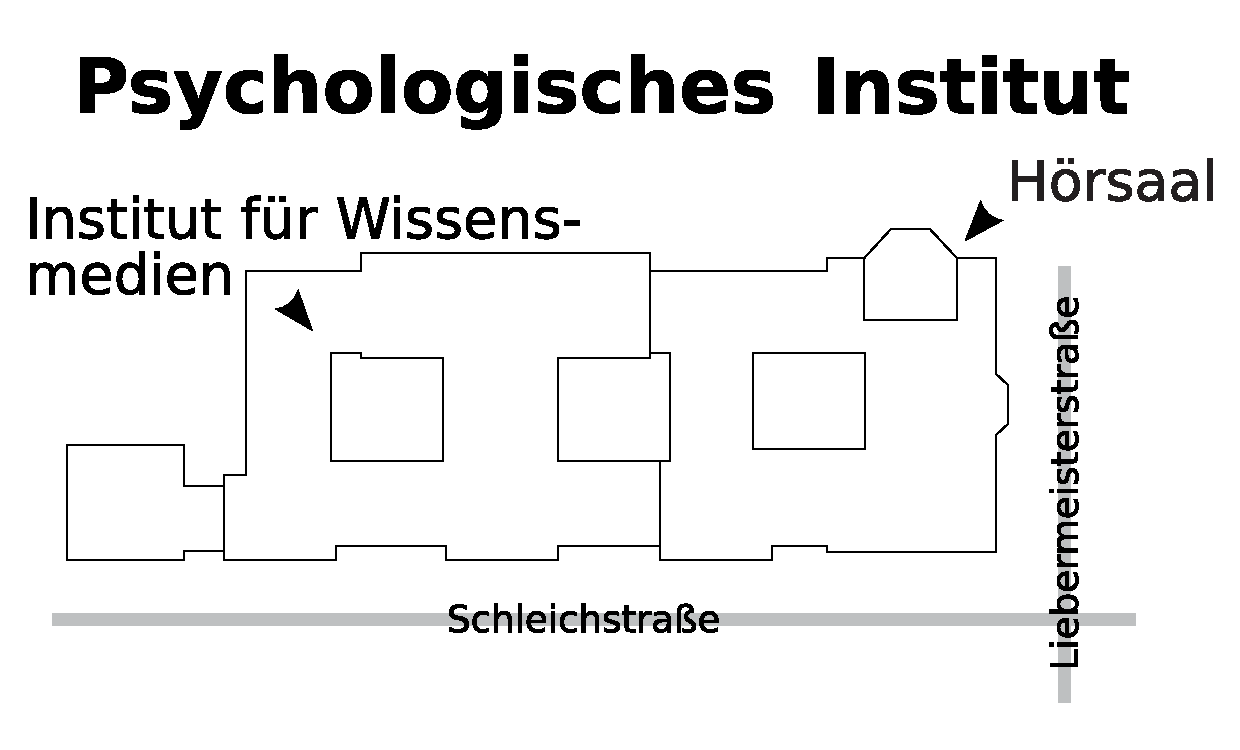
\includegraphics[width=\linewidth]{pictures/uebersicht_pi.pdf}\\
			\end{column}
		\end{columns}
	\end{frame}
	
	\begin{frame}
		\begin{columns}
			\column{0.6\textwidth}
			
\includegraphics[width=\textwidth]{pictures/keepcalm.pdf}
			\column{0.4\textwidth}
			\centering
			\begin{huge}
				Wir freuen uns auf euch! \vspace*{1cm}
			\end{huge}
			
			\qrcode{https://www.fsi.uni-tuebingen.de}\\
			\begin{scriptsize}
				https://www.fsi.uni-tuebingen.de
			\end{scriptsize}
		\end{columns}
		
	\end{frame}

\end{document}
